\documentclass[12pt]{article}


\usepackage{graphicx}
\usepackage{caption}
\usepackage{float}
\usepackage{subcaption}

\usepackage{amsmath}
\usepackage{algorithm}
\usepackage[noend]{algpseudocode}

\makeatletter
\def\BState{\State\hskip-\ALG@thistlm}
\makeatother

\usepackage[hidelinks]{hyperref}


\usepackage[nameinlink]{cleveref}
\AtBeginDocument{%
  \crefname{equation}{برابری}{equations}%
  \crefname{chapter}{فصل}{chapters}%
  \crefname{section}{بخش}{sections}%
  \crefname{appendix}{پیوست}{appendices}%
  \crefname{enumi}{مورد}{items}%
  \crefname{footnote}{زیرنویس}{footnotes}%
  \crefname{figure}{شکل}{figures}%
  \crefname{table}{جدول}{tables}%
  \crefname{theorem}{قضیه}{theorems}%
  \crefname{lemma}{لم}{lemmas}%
  \crefname{corollary}{نتیجه}{corollaries}%
  \crefname{proposition}{گزاره}{propositions}%
  \crefname{definition}{تعریف}{definitions}%
  \crefname{result}{نتیجه}{results}%
  \crefname{example}{مثال}{examples}%
  \crefname{remark}{نکته}{remarks}%
  \crefname{note}{یادداشت}{notes}%
  \crefname{observation}{مشاهده}{observations}%
  \crefname{algorithm}{الگوریتم}{algorithms}%
  \crefname{cproof}{برهان}{cproofs}%
}

\usepackage{xepersian}

\settextfont{XB Zar}[
  Path=./fonts/,
  Scale=1.2,
  Extension=.TTF,
  UprightFont=*,
  ItalicFont=*It,
  BoldFont=*Bd,
  BoldItalicFont=*BdIt
]

\setdigitfont{XB Zar}[
  Path=./fonts/,
  Scale=1.2,
  Extension=.TTF,
  UprightFont=*,
  ItalicFont=*It,
  BoldFont=*Bd,
  BoldItalicFont=*BdIt
]

\setlatintextfont[Scale=1.1]{Times New Roman}

% \setmonofont[
%   Path=./fonts/,
%   Scale=1.0,
%   Weight=800,
%   Extension=.TTF,
% ]{Inconsolata}


\title{مقایسه الگوریتم‌های مرتب‌سازی}
\author{محمد ترابی - علی جعفر‌آبادی - رضا تاج‌گذاری} 
\date{تیرماه ۱۴۰۲}

\begin{document}
\maketitle

\pagebreak

\section{مرتب‌سازی درجی\protect\LTRfootnote{insertion sort}}

اگر یک دسته کارت به شما داده شود که اعداد ۱ تا ۵۰ روی آن نوشته شده است، چگونه آن را مرتب
\LTRfootnote{sort}
می‌کنید؟
احتمالا اول تعداد کمی کارت برمی‌دارید و آن را مرتب می‌کنید؛
سپس بقیه کارت‌ها را یکی پس از دیگری نگاه می‌کنید
و در جای مناسب میان کارت‌های مرتب شده قرار می‌دهید.
\cref{fig:f1}
نمایی کلی از این روش مرتب‌سازی نشان می‌دهد.

وقتی کارت‌ها را با این روند مرتب می‌کنیم،
همواره تعدادی از کارت‌ها مرتب شده است و کارت‌هایی که هنوز مرتب نشده، یکی پس از دیگری
در دستهٔ کارت‌های مرتب شده درج
\LTRfootnote{insert}
می‌شوند.
اگر با این روش کارت‌ها را مرتب کنیم، درواقع از مرتب‌سازی درجی استفاده کرده ایم.

\begin{figure}[H]
  \centering
  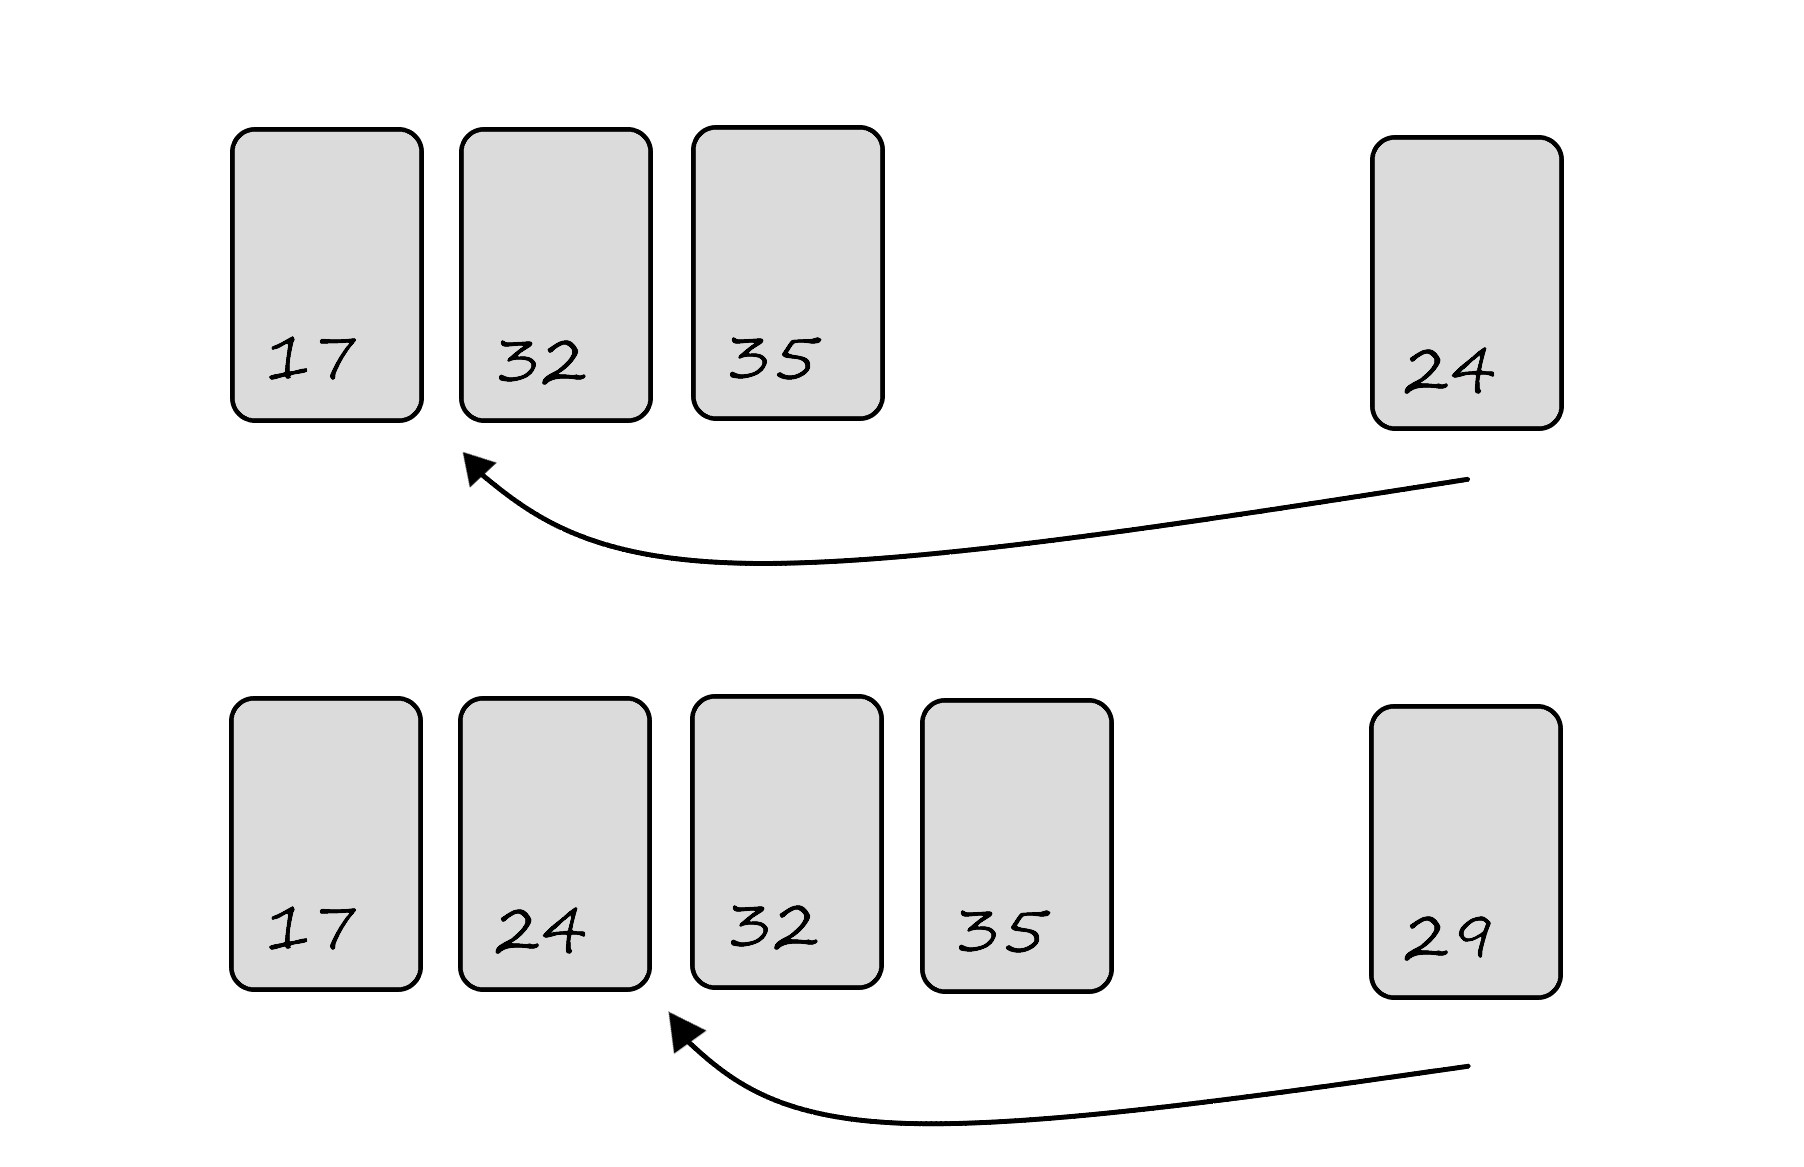
\includegraphics[width=.8\textwidth]{figs/sortingCards2.jpg}
  \caption{
    مرتب کردن کارت‌ها به کمک مرتب‌سازی درجی
  }
  \label{fig:f1}
\end{figure}

\subsection*{الگوریتم مرتب‌سازی درجی}
آرایه‌ای به طول یک همواره مرتب است؛ بنابراین از عنصر دوم شروع می‌کنیم و جلو می‌رویم.
فرض کنیم که به عنصر
$i$
رسیده‌ایم،
عناصر قبل از
$i$
مرتب‌اند.
لذا از آخرین عنصر قبل از
$i$
شروع می‌کنیم و
هر یک از عناصر بزرگتر از
$i$
را یک واحد به سمت راست انتقال
\LTRfootnote{shift}
می‌دهیم.
وقتی به عنصری کوچک تر از
$i$
یا به ابتدای آرایه رسیدیم
متوقف می‌شویم و
$i$
را همانجا درج
می‌کنیم.
شبه‌کد مرتب‌سازی درجی را می‌توانید در
\cref{alg:a1}
که در ادامه آمده است
مشاهده کنید
\footnote{
  توجه داشته باشید که الگوریتم بر پایه صفر است؛ یعنی عنصر اول آرایه
  $arr[0]$
  می‌باشد.
}
.

\begin{algorithm}[H]
  \caption{مرتب‌سازی درجی}
  \begin{latin}
    \begin{algorithmic}[1]
      \Procedure{InsertionSort}{arr, n}
      \For {$i \leftarrow 1$ \textbf{to} $n-1$}
      \State $key \gets arr[i]$
      \State $j \gets i-1$
      \While {$j >= 0$ and $arr[j] > key$}
      \State $arr[j+1] \gets arr[j]$
      \State $j \gets j - 1$
      \EndWhile
      \State $arr[j+1] \gets key$
      \EndFor
      \EndProcedure
    \end{algorithmic}
  \end{latin}
  \label{alg:a1}
\end{algorithm}

اگر الگوریتم بالا را روی آرایهٔ
$[7, 6, 6, 4, 9]$
اجرا کنیم،
آرایه بدین صورت مرتب می‌شود:
\begin{align*}
   & [7, 6, 6, 4, 9] \rightarrow [7, 7, 6, 4, 9] \rightarrow
  [6, 7, 6, 4, 9] \rightarrow [6, 7, 7, 4, 9] \rightarrow    \\
   & [6, 6, 7, 4, 9] \rightarrow [6, 6, 7, 7, 9] \rightarrow
  [6, 6, 6, 7, 9] \rightarrow [6, 6, 6, 7, 9]  \rightarrow   \\
   & [4, 6, 6, 7, 9] \rightarrow [4, 6, 6, 7, 9]
\end{align*}

توجه داشته باشید که پیچیدگی زمانی مرتب‌سازی درجی در بهترین حالت خطی است.
همچنین بهترین حالت وقتی اتفاق می‌افتد که آرایه مرتب باشد.
می‌توانیم نتیجه بگیریم که در مواقعی که آرایه مرتب و یا تقریبا مرتب است
مرتب‌سازی درجی بسیار سریع عمل می‌کند.
بنابراین اگر از قبل مطلع هستیم که معمولا داده‌های ما تقریبا مرتب است، استفاده از مرتب‌سازی درجی
می‌تواند گزینه مناسبی باشد.

به عنوان مثال فرض کنید که یک لیست هزارتایی از اسامی دانشجویان یک موسسه در اختیار دارید که به ترتیب حروف الفبا مرتب شده اند.
در سال جدید پنجاه دانشجو در موسسه نام نویسی می‌کنند و اسامی آن‌ها به آخر آرایه اضافه می‌شود.
اگرچه روش‌های زیادی برای مرتب کردن لیست جدید دانشجویان وجود دارد، مرتب‌سازی درجی گزینه مناسبی محسوب می‌شود
و از دیگر روش‌های مرتب‌سازی که در این مقاله توضیح داده شده، بهتر عمل می‌کند.

خوب است بدانیم
می‌توان پیچیدگی زمانی مرتب سازی درجی را با تغییرات کمی بهبود بخشید
که در این مقاله به آن نمی‌پردازیم.
به عنوان مثال مرتب‌سازی شِل
\LTRfootnote{shell sort}
یک روش مرتب سازی است که از مرتب‌سازی درجی الهام گرفته شده
و از نظر پیچیدگی زمانی از مرتب‌سازی درجی بهتر عمل می‌کند.
\cite{shell1}
\cite{shell2}

{
\fontsize{12pt}{10pt}\selectfont
\bibliographystyle{ieeetr-fa}
\bibliography{refs}
\addcontentsline{toc}{section}{مراجع}
}

\end{document}